
由于CPU上有多种代码执行的机制,所以会造成一些混乱,如图2-16所示。\par

CPU最直接执行的还是主机代码,要么是单源应用程序的一部分(主机代码区域),要么是主机代码对其他主机代码或库(如库函数)的调用。\par

其他两个设备用于径执行设备代码。第一段设备代码在CPU上是通过主机执行,这种方式在本章前面已经了解过。\par

SYCL在CPU上执行设备代码的第二种可选方式是,使用CPU加速器对性能进行优化。该设备通常由OpenCL等底层运行时库实现,因此其可用性需要依赖于系统上安装的驱动程序和其他运行时库。SYCL中,主机设备旨在通过本机CPU工具对设备代码进行调试,而CPU作为设备时,设备代码会运行在对性能有优化的实现上。\par

\hspace*{\fill} \par %插入空行
图2-16 SYCL在CPU上的执行机制
\begin{center}
	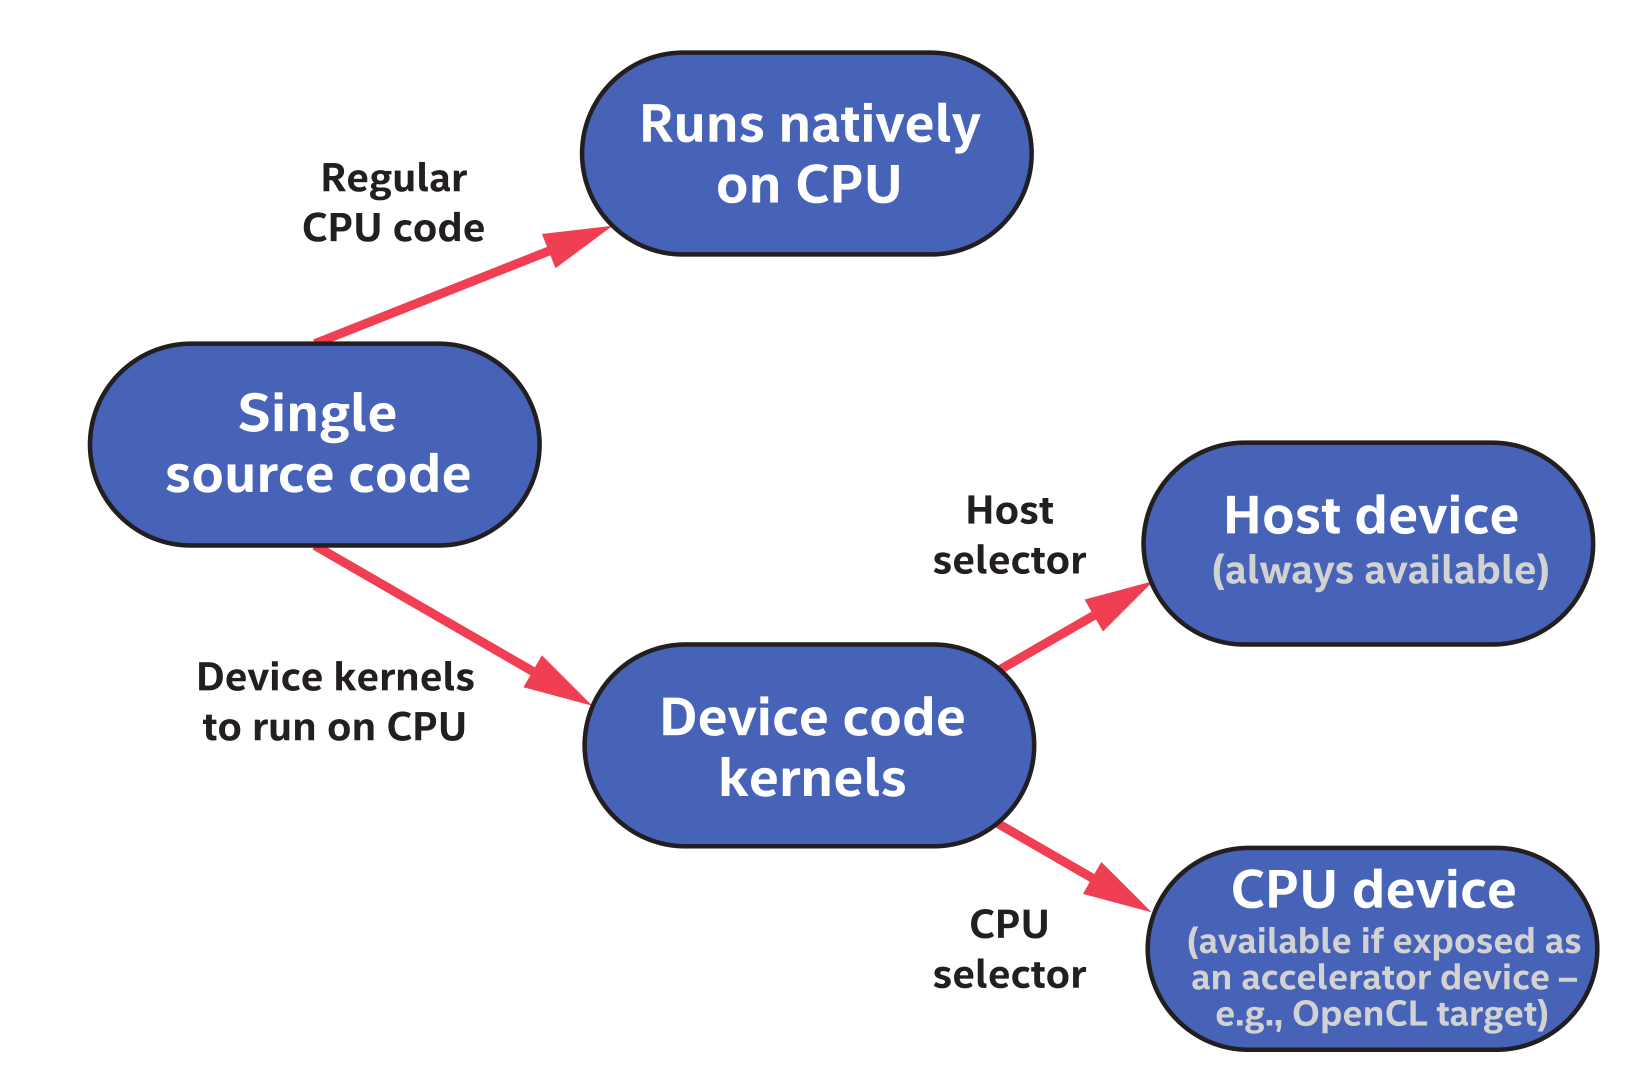
\includegraphics[width=0.7\textwidth]{content/chapter-2/images/9}
\end{center}

有一种机制本书没有涉及,可以在满足任务图中的先决条件时,将常规CPU代码(图2-16的顶部部分)进行入队。这个特性可以用来执行在任务图中的常规CPU代码和设备代码,也称为主机任务。\par








